% !TeX root = orbits.tex
% !TeX Program=pdfLaTeX

%%%%%%%%%%%%%%%%%%%%%%%%%%%%%%%%%%%%%%%%%%%%%%%%%%%%%%%%%%%%%%%%

\chapter{Elliptical orbits}\label{s.kepler}

Towards the end of the sixteenth century, the astronomer Tycho Brahe carried out extremely precise observations. In 1600 he hired Johannes Kepler as his assistant and when Tycho died soon afterwards, Kepler was appointed to his position. Here we explain how Kepler was able to establish that planetary orbits are ellipses.

\section{Determining the radius of the Earth's orbit}

A Martian year is $687$ days, that is, it equals $\frac{687}{365.25} = 1.88$ Earth years. We know when Mars reaches a ``new year'' by observing its projection on the celestial sphere, but each time the position of the Earth in its orbit will be different. Figure~\ref{f.kepler-mars} shows the orbit of the Earth---its center $O$ offset from the Sun $S$ as Copernicus showed---at four occasions when the position of Mars $M$ at its new year was observed. Four triangles are created $\triangle OE_iM$.

%%%%%%%%%%%%%%%%%%%%%%%%%%%%%%%%%%%%%%%%%%%%%%%%%%%%%%%%%%%%

\begin{figure}[b]
\begin{center}
\begin{tikzpicture}[scale=.8]

\clip (-2.8,-3) rectangle +(8,6);

% The center of the Earth's orbit
\coordinate (O) at (0,0);
\node[below left] at (O) {$O$};

% The circular orbit of the Earth and an arc of the orbit of Mars
\draw[name path=Eorbit] (O) circle[radius=2.5cm];
\draw ($(O)+(-35:5)$) arc[start angle=-35,end angle=35,radius=5cm];

% Locate Mars
\coordinate (M) at (-25:5);
\node[right] at (M) {$M$};

% Draw common side OM
\draw[thick] (O) -- (M);

% Locate various positions of the Earth in its orbit
\foreach \angle/\name/\c in { 110/E1/red, 70/E2/purple, 25/E3/{blue}, -40/E4/green} {
  \coordinate (\name) at (\angle:2.5);
  %\vertexsmcolor{\name}{\c};
  \draw[\c,thick] (O) -- (\name) -- (M);
}

% Label the Earth's positions
\node[above,yshift=1pt] at (E1) {$E_1$};
\node[above] at (E2) {$E_2$};
\node[right,xshift=2pt] at (E3) {$E_3$};
\node[below,xshift=2pt,yshift=-3pt] at (E4) {$E_4$};

% Nodes drawn at the end to override colors
%\vertexsm{M};
%\vertexsm{O};

% Draw the Sun
\coordinate (S) at (25:20pt);
\vertexsm{S};
\node[right,yshift=-3pt] at (S) {$S$};

\end{tikzpicture}
\caption{Observations of the orbit of Mars from the Earth}\label{f.kepler-mars}
\end{center}
\end{figure}

%%%%%%%%%%%%%%%%%%%%%%%%%%%%%%%%%%%%%%%%%%%%%%%%%%%%%%%%%%%%

Figure~\ref{f.kepler-one-triangle} shows one of the triangles with the angles labeled. Using the law of sines,
\begin{eqn}
\frac{OE_i}{\sin \beta} &=& \frac{OM}{\sin \alpha}\\[4pt]
OE_i &=& OM\,\frac{\sin \beta}{\sin \alpha}\,.
\end{eqn}%

%%%%%%%%%%%%%%%%%%%%%%%%%%%%%%%%%%%%%%%%%%%%%%%%%%%%%%%%%%%%

\begin{figure}[t]
\begin{center}
\begin{tikzpicture}[scale=.8]

\clip (-2.7,-2.7) rectangle +(8,6);

% The center of the Earth's orbit
\coordinate (O) at (0,0);
\node[below left] at (O) {$O$};

% The circular orbit of the Earth and an arc of the orbit of Mars
\draw[name path=Eorbit] (O) circle[radius=2.5cm];
\draw ($(O)+(-35:5)$) arc[start angle=-35,end angle=35,radius=5cm];

% Locate Mars
\coordinate (M) at (-25:5cm);
\node[right] at (M) {$M$};

% Draw one triangle
\coordinate (E2) at (70:2.5cm);
\node[above] at (E2) {$E_i$};
\draw[thick] (O) -- (E2) -- (M) -- cycle;

% Label the vertices
\vertexsm{O};
\vertexsm{E2};
\vertexsm{M};
\node[right,xshift=4pt,yshift=4pt] at (O) {$\alpha$};
\node[above left,xshift=-20pt,yshift=14pt] at (M) {$\beta$};
\node[below,xshift=2pt,yshift=-8pt] at (E2) {$\gamma$};

\end{tikzpicture}
\caption{One triangle Earth-Sun-Moon}\label{f.kepler-one-triangle}
\end{center}
\end{figure}

%%%%%%%%%%%%%%%%%%%%%%%%%%%%%%%%%%%%%%%%%%%%%%%%%%%%%%%%%%%%

Tycho Brahe measured all three angles and the values of $OE_i$ given in the fourth column of the table are not equal. If the Earth' orbit is circular, he had to move the center of the orbit so that $\{E_1,E_2,E_3,E_4\}$ were all on the circle.

\section{Measuring the angles in the triangle Sun-Earth-Mars}


\begin{wrapfigure}[7]{R}{.5\textwidth}
\[
\begin{array}{rrrrr}
\hline
& \multicolumn{1}{c}{\alpha} & \multicolumn{1}{c}{\beta} &
  \multicolumn{1}{c}{\gamma} & \multicolumn{1}{c}{OE_i} \\\hline
E_1 & 127.1 & 20.8  & 32.1 & \;\; 0.6682\cdot OM\\
E_2 & 84.2 & 35.8 & 60.5 & \;\;0.6721\cdot OM\\
E_3 & 41.3 & 42.4 &96.4 & \;\;0.6785\cdot OM\\
E_4 & 1.6& 3.4& 175.0 & \;\;0.6805\cdot OM\\
\hline
\end{array}
\]
\end{wrapfigure}

How can the angles $\alpha, \beta, \gamma$ be measured? $\triangle E_iOM$ is a triangle so it is sufficient to measure two of the angles. $\gamma$ is easily measured by observing Mars and the Sun at the same time, but neither $\alpha$ nor $\beta$ can be measured directly since they are not accessible to an observer on Earth.

Tycho's measurement used the known periods of the orbits to compute the angles. The Earth moves counterclockwise around Sun. Given any point $E$, for some $t$, $t$ days later the Earth will have moved to $E'$ and Mars will have moved to $M'$, so that they are in \emph{opposition}, that is, Mars will be on the continuation of the Earth-Sun line (Figure~\ref{f.kepler-opposition}). Since the Earth completes an orbit in about half the time that Mars takes to complete an orbit, $t$ will be such that neither the Earth nor Mars has completed a full orbit. The angles $\theta_E$ and $\theta_M$ are fractions of a circular orbit of $360^\circ$, so
%
%%%%%%%%%%%%%%%%%%%%%%%%%%%%%%%%%%%%%%%%%%%%%%%%%%%%%%%%%%%%
%
\begin{figure}[b]
\begin{minipage}{.48\textwidth}
\begin{center}
\begin{tikzpicture}[scale=.8]

\clip (-3.5,-2.6) rectangle +(9,6.2);

% The center of the Earth's orbit
\coordinate (O) at (0,0);
\node[below] at (O) {$O$};

% The circular orbit of the Earth and an arc of the orbit of Mars
\draw[name path=Eorbit] (O) circle[radius=2.5cm];
\draw ($(O)+(-35:5)$) arc[start angle=-35,end angle=35,radius=5cm];

% Locate Mars
\coordinate (M) at (-25:5);
\node[right] at (M) {$M$};

% Draw one triangle
\coordinate (E2) at (70:2.5);
\node[above] at (E2) {$E$};
\draw (O) -- (E2) -- (M) -- cycle;

% Label angles of the triangle
\node[right,xshift=6pt,yshift=16pt] at (O) {\sm{\alpha\!-\!\theta_M}};
\node[above left,xshift=-20pt,yshift=14pt] at (M) {$\beta$};
\node[below,xshift=2pt,yshift=-8pt] at (E2) {$\gamma$};

% Label angles at the center of the Earth's orbit
\draw ($(O)+(-25:.5)$) arc[start angle=-25,end angle=20,radius=.5cm];
\node[right,xshift=12pt,yshift=-1pt] at (O) {$\theta_M$};
\draw ($(O)+(20:.5)$) arc[start angle=20,end angle=70,radius=.5cm];
\node[right,xshift=12pt,yshift=-1pt] at (O) {$\theta_M$};
\draw ($(O)+(70:.5)$) arc[start angle=70,end angle=200,radius=.5cm];
\node[above left,xshift=-4pt,yshift=10pt] at (O) {$\theta_E$};

% Locate E'
\coordinate (E2P) at (200:2.5);
\node[left] at (E2P) {$E'$};
\coordinate (MPP) at (20:5);
\vertexsm{MPP};
\node[above right] at (MPP) {$M'$};
\draw[thick] (E2P) -- (MPP);

% Draw arc for t from E to E'
\draw[->,dashed,thick] (70:3.2) 
   arc[start angle=70,end angle=200,radius=3.3]
   node[above,midway] {$t$};

\end{tikzpicture}
\caption{The Earth and Mars in opposition\\\mbox{}}\label{f.kepler-opposition}
\end{center}
\end{minipage}
\hspace*{12pt}
\begin{minipage}{.48\textwidth}
\begin{center}
\begin{tikzpicture}[scale=.8]

\clip (-2.9,-2.6) rectangle +(8.3,6.2);

% The center of the Earth's orbit
\coordinate (O) at (0,0);
\vertexsm{O};
\node[below left] at (O) {$O$};

% The circular orbit of the Earth and an arc of the orbit of Mars
\draw[name path=Eorbit] circle[radius=2.5cm];
\draw ($(O)+(-35:5)$) arc[start angle=-35,end angle=35,radius=5cm];

% Locate Mars
\coordinate (M) at (-25:5);
\node[right] at (M) {$M$};

% Draw the Sun
\coordinate (S) at (25:30pt);
\vertexsm{S};
\node[right,yshift=-3pt] at (S) {$S$};

% Draw the center of the new orbit
\coordinate (OP) at (25:12pt);
%\vertexsm{OP};
\node[below,yshift=-2pt] at (OP) {$O'$};
\draw (O) -- (OP);

% Draw new orbit
\draw[name path=Eorbitnew,dashed,thick] (OP) circle[radius=2.5cm];

% Draw common side OM
\draw[thick] (OP) -- (M);

% Locate various positions of the Earth in its orbit
\foreach \angle/\name/\c in { 110/E1/red, 70/E2/purple, 25/E3/{blue}, -40/E4/green} {
  \coordinate (\name) at ($(OP)+(\angle:2.5)$);
  %\vertexsmcolor{\name}{\c};
  \draw[\c,thick] (OP) -- (\name) -- (M);
}

% Label the Earth's positions
\node[above left,yshift=1pt] at (E1) {$E_1$};
\node[above right] at (E2) {$E_2$};
\node[right,xshift=2pt] at (E3) {$E_3$};
\node[below,xshift=2pt,yshift=-3pt] at (E4) {$E_4$};

% Nodes drawn at the end to override colors
%\vertexsm{M};
\vertexsm{OP};

\end{tikzpicture}
\caption{Observations of the orbit of Mars from the new Earth's orbit}\label{f.kepler-earth-new}
\end{center}
\end{minipage}
\end{figure}

%%%%%%%%%%%%%%%%%%%%%%%%%%%%%%%%%%%%%%%%%%%%%%%%%%%%%%%%%%%%
%
\begin{eqn}
\frac{t}{365.25} &=& \frac{\theta_E}{360}\\[2pt]
\theta_E &=& \frac{360}{365.35}t\\[2pt]
\frac{t}{687} &=& \frac{\theta_M}{360}\\[2pt]
\theta_M &=& \frac{360}{687}t\,.
\end{eqn}

This gives values for $\theta_E$ and $\theta_M$. Since $E'M'$ is a straight line, we have that $\alpha-\theta_M = 180^\circ -\theta_E$, so that $\alpha = 180 - \theta_E + \theta_M$, and the values of $OE_i$ can be computed.

\section{A new location for the center of the Earth's orbit}

Kepler's next task was to obtain a new value $O'$ for the center of the Earth's orbit such that the $E_i$'s are on the orbit. Given the new locations of the Earth $\{E_1,E_2,E_3,E_4\}$, by Theorem~\ref{thm.three-points} a circle centered at $O'$ can be constructed that goes through $\{E_1,E_2,E_3\}$ (Figure~\ref{f.kepler-earth-new}). To verify that this is the correct orbit, check that $E_4$ is on the circle.

%%%%%%%%%%%%%%%%%%%%%%%%%%%%%%%%%%%%%%%%%%%%%%%%%%%%%%%%%%%%

%\begin{figure}[b]
%\begin{center}
%\begin{tikzpicture}[scale=.8]
%
%\clip (-2.8,-3) rectangle +(8,6.2);
%
%% The center of the Earth's orbit
%\coordinate (O) at (0,0);
%\vertexsm{O};
%\node[below left] at (O) {$O$};
%
%% The circular orbit of the Earth and an arc of the orbit of Mars
%\node[draw,circle,minimum size=5cm,name path=Eorbit] at (O) {};
%\draw ($(O)+(-35:5)$) arc[start angle=-35,end angle=35,radius=5cm];
%
%% Locate Mars
%\coordinate (M) at (-25:5);
%\node[right] at (M) {$M$};
%
%% Draw the Sun
%\coordinate (S) at (25:30pt);
%\vertexsm{S};
%\node[right,yshift=-3pt] at (S) {$S$};
%
%% Draw the center of the new orbit
%\coordinate (OP) at (25:12pt);
%%\vertexsm{OP};
%\node[below,yshift=-2pt] at (OP) {$O'$};
%\draw (O) -- (OP);
%
%% Draw new orbit
%\node[draw,thick,dashed,circle,minimum size=5cm,
%      name path=Eorbitnew] at (OP) {};
%
%% Draw common side OM
%\draw[thick] (OP) -- (M);
%
%% Locate various positions of the Earth in its orbit
%\foreach \angle/\name/\c in { 110/E1/red, 70/E2/purple, 25/E3/{blue}, -40/E4/green} {
%  \coordinate (\name) at ($(OP)+(\angle:2.5)$);
%  %\vertexsmcolor{\name}{\c};
%  \draw[\c,thick] (OP) -- (\name) -- (M);
%}
%
%% Label the Earth's positions
%\node[above left,yshift=1pt] at (E1) {$E_1$};
%\node[above right] at (E2) {$E_2$};
%\node[right,xshift=2pt] at (E3) {$E_3$};
%\node[below,xshift=2pt,yshift=-3pt] at (E4) {$E_4$};
%
%% Nodes drawn at the end to override colors
%%\vertexsm{M};
%\vertexsm{OP};
%
%\end{tikzpicture}
%\caption{Observations of the orbit of Mars from the new Earth's orbit}\label{f.kepler-earth-new}
%\end{center}
%\end{figure}

%%%%%%%%%%%%%%%%%%%%%%%%%%%%%%%%%%%%%%%%%%%%%%%%%%%%%%%%%%%%

\section{Orbits are ellipses}

While Kepler was able to modify the center of the orbit of the Earth to be consistent with the observations, he was not able to adequately describe the orbit of Mars. After years of work, he came to the conclusion that the orbit must be oval like an egg. Oval, perhaps, but certainly not an ellipse, because ``the job would have been done by Archimedes \cite[p.~94]{hahn-cic}.'' Figure~\ref{f.kepler-egg} shows $C$, a position on a circular orbit, and an oval orbit (dashed), where $M$ is the position of Mars on the oval corresponding to $C$. The radius of the circular orbit is labeled $a=OA=OC$ and the unknown distances to $M$ are labeled $s=SM$ and $t=OM$.

Kepler's computed that $\frac{a-t}{t} = 0.00429$ and $\frac{s}{t} = 1.00429$, so that $(a-t)+t=s$
%\begin{eqn}
%\frac{a-t}{t} &=& \frac{s}{t}-1\\[4pt]
%a-t &=& s-t\,,
%\end{eqn}%%
and therefore $SM=s=a=AO$. The dashed oval is likely an ellipse, because in an ellipse $SM=AO$ (Theorem~\ref{thm.ellipses-features}). Kepler then computed the projections of the observations of Mars on the $x$-axis (Figure~\ref{f.kepler-ellipse}) and obtained for all of them that
\[
\frac{M_iO_i}{C_iO_i} = \frac{1}{1.00429}=0.99573\,.
\]
By Theorem~\ref{thm.ellipse-b-over-a}, $MO/CO=b/a$ is constant for an ellipse, and Kepler concluded that the orbit of Mars is an ellipse.

%%%%%%%%%%%%%%%%%%%%%%%%%%%%%%%%%%%%%%%%%%%%%%%%%%%%%%%%%%%%

\begin{figure}[t]
\begin{minipage}{.48\textwidth}

\begin{center}
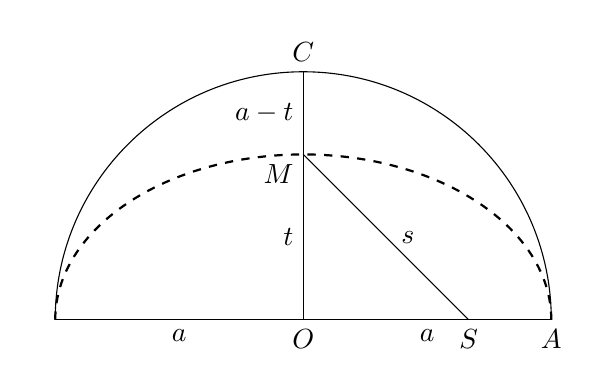
\begin{tikzpicture}[scale=.7]

\clip (-5,-.7) rectangle +(10,6);

% The center of the Earth's orbit
\coordinate (O) at (0,0);
\node[below] at (O) {$O$};
%\vertexsm{O};
\coordinate (C) at (0,4.5);
\coordinate (A) at (4.5,0);

% The circular orbit of the Earth and an elliptical orbit of Mars
\draw[thick,dashed] (A) arc(0:180:4.5cm and 3cm);
\draw (4.5,0) arc(0:180:4.5cm);
\draw (0,0) -- (C) node[above] {$C$};
\draw (-4.5,0) -- node[below] {$a$} (O) -- 
  node[below,xshift=0pt] {$a$} (A) node[below] {$A$};

% Locate Mars
\coordinate (M) at (0,3);
\node[below left] at (M) {$M$};
%\vertexsm{M};

% Locate the Sun
\coordinate (S) at (3,0);
%\vertexsm{S};
\node[below] at (S) {$S$};

% Draw line from Sun to Mars
\draw (M) -- node[right,xshift=2pt] {$s$} (S);
\path (O) -- node[left] {$t$} (M) -- node[left] {$a-t$} (C);

\end{tikzpicture}
\caption{The orbit of Mars as an oval ``egg''}\label{f.kepler-egg}
\end{center}
\end{minipage}
%%%%%%%%%%%%%%
\begin{minipage}{.48\textwidth}
\begin{center}
\begin{tikzpicture}[scale=.7]
\clip (-5,-.7) rectangle +(10,6);

% The center of the Earth's orbit
\coordinate (O) at (0,0);
\node[below] at (O) {$O$};
\coordinate (C) at (0,4.5);
\coordinate (A) at (4.5,0);

% The circular orbit of the Earth and an elliptical orbit of Mars
\draw[name path=ellipse,thick,dashed] (A) arc(0:180:4.5cm and 3cm);
\draw[name path=circle] (4.5,0) arc(0:180:4.5cm);
\draw (0,0) -- (C) node[above] {$C$};
\draw (-4.5,0) --  (O) -- (A);

% Locate Mars
\coordinate (M) at (0,3);
\node[below left] at (M) {$M$};

% Locate the projections
\coordinate (O1) at (-3,0);
\node[below] at (O1) {$O_1$};
\coordinate (O2) at (-1,0);
\node[below] at (O2) {$O_2$};
\coordinate (O3) at (1.8,0);
\node[below] at (O3) {$O_3$};

% Get intersections with the circle
\path[name path=P1] (O1) -- +(0,4.5);
\path[name path=P2] (O2) -- +(0,4.5);
\path[name path=P3] (O3) -- +(0,4.5);

\path [name intersections = {of = circle and P1, by = {C1} }];
\path [name intersections = {of = circle and P2, by = {C2} }];
\path [name intersections = {of = circle and P3, by = {C3} }];

% Get intersections with the ellipse
\path [name intersections = {of = ellipse and P1, by = {M1} }];
\path [name intersections = {of = ellipse and P2, by = {M2} }];
\path [name intersections = {of = ellipse and P3, by = {M3} }];

\draw (O1) -- (C1) node[above,yshift=4pt] {$C_1$};
\draw (O2) -- (C2) node[above] {$C_2$};
\draw (O3) -- (C3) node[above] {$C_3$};

% Label positions of Mars on the ellipse
%\vertexsm{M1};
\node[below right] at (M1) {$M_1$};
%\vertexsm{M2};
\node[below left,yshift=-4pt,xshift=1pt] at (M2) {$M_2$};
%\vertexsm{M3};
\node[below left] at (M3) {$M_3$};
\end{tikzpicture}
\caption{The orbit of Mars as an ellipse}\label{f.kepler-ellipse}
\end{center}
\end{minipage}
\end{figure}
